\chapter*{Appendix}
\addcontentsline{toc}{chapter}{Appendix}

\subsection{Подробная архитектура 150M Llama-like модели}\label{app:architecture_150m_llama}

При обучении с нуля была использована следующая конфигурация Llama-like модели:
\begin{enumerate}
    \item \texttt{hidden\_size} = 768
    \item \texttt{intermediate\_size} = 3072
    \item \texttt{num\_hidden\_layers} = 12
    \item \texttt{num\_attention\_heads} = 12
    \item \texttt{num\_key\_value\_heads} = 12
    \item \texttt{head\_dim} = 64
    \item \texttt{rope\_theta} = 50000
    \item \texttt{max\_seq\_len} = 1024
    \item \texttt{torch\_dtype} = \texttt{bfloat16}
    \item \texttt{attn\_implementation} = \texttt{flash\_attention\_2}
\end{enumerate}


\begin{figure}[h]
    \centering
    \begin{minipage}{0.48\textwidth}
        \centering
        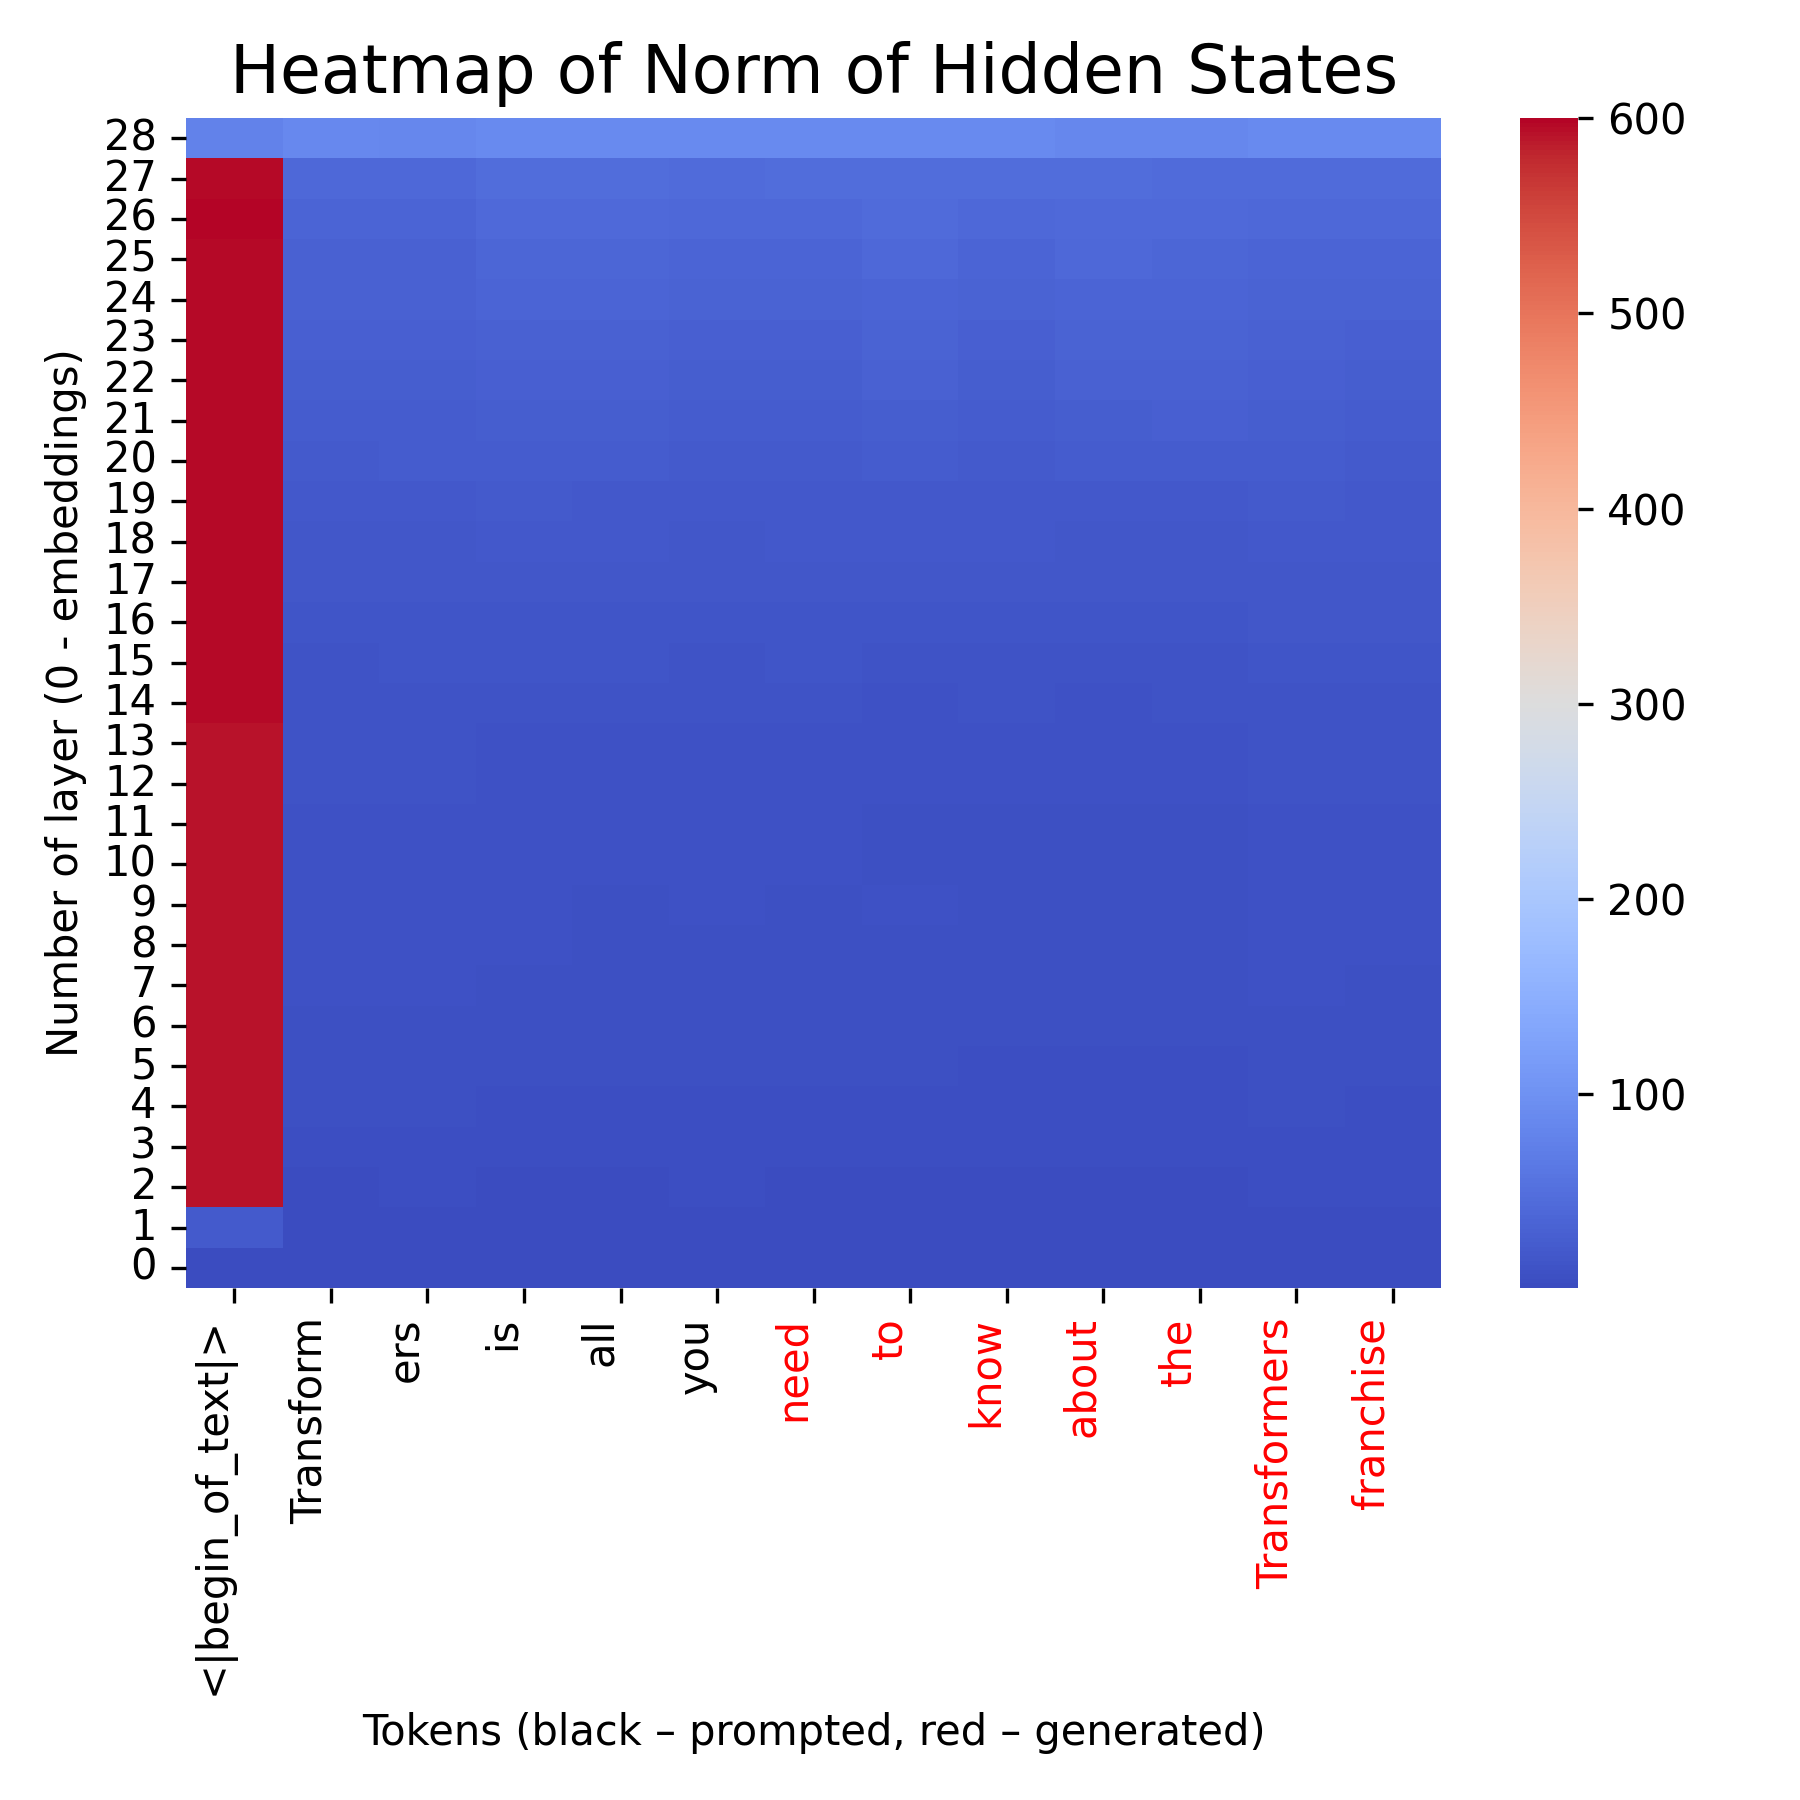
\includegraphics[width=\textwidth]{images/heatmap_3b_full.png}
        \caption{Heatmap of hidden state norms across layers and tokens for Llama 3.2 3B model. The x-axis represents tokens in the sequence (with generated tokens in red), and the y-axis represents model layers (with 0 being the embedding layer). Brighter colors indicate larger norms.}
        \label{fig:heatmap_3b_full}
    \end{minipage}
    \hfill
    \begin{minipage}{0.48\textwidth}
        \centering
        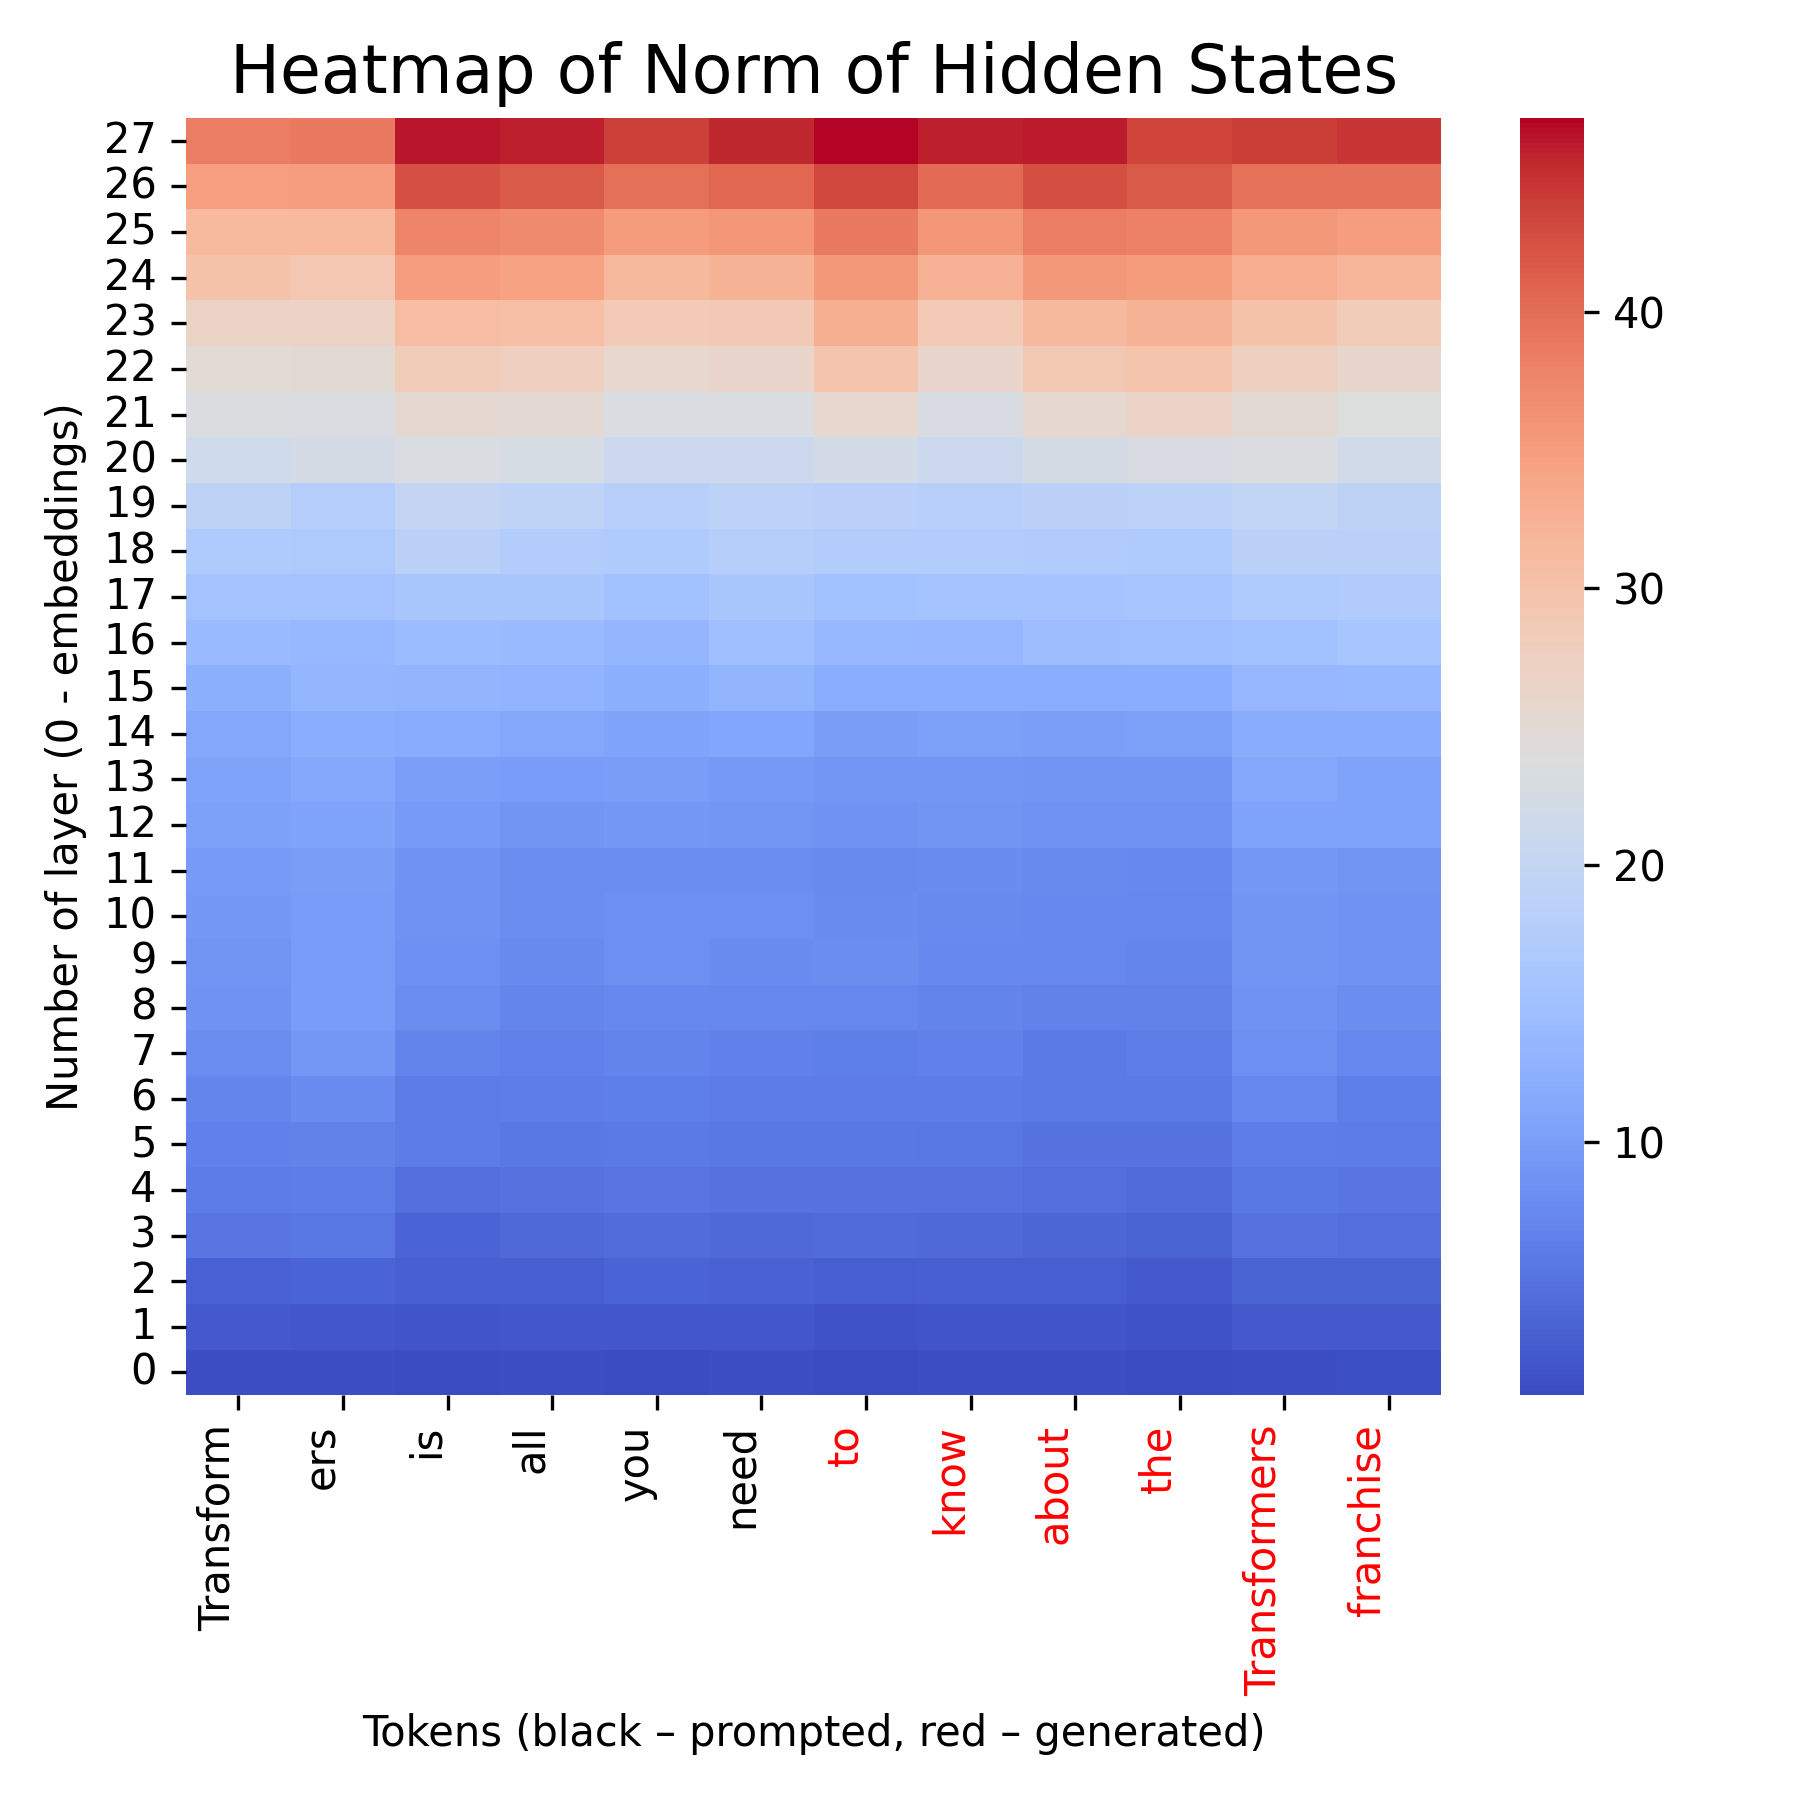
\includegraphics[width=\textwidth]{images/heatmap_3b_notfull.png}
        \caption{Heatmap of hidden state norms excluding the <BOS> token and final layer for Llama 3.2 3B model, providing a clearer view of the norm distribution in intermediate layers. Note the gradual increase in norm magnitude as layer depth increases.}
        \label{fig:heatmap_3b_notfull}
    \end{minipage}
\end{figure}


\begin{figure}[h]
    \centering
    \begin{minipage}{0.48\textwidth}
        \centering
        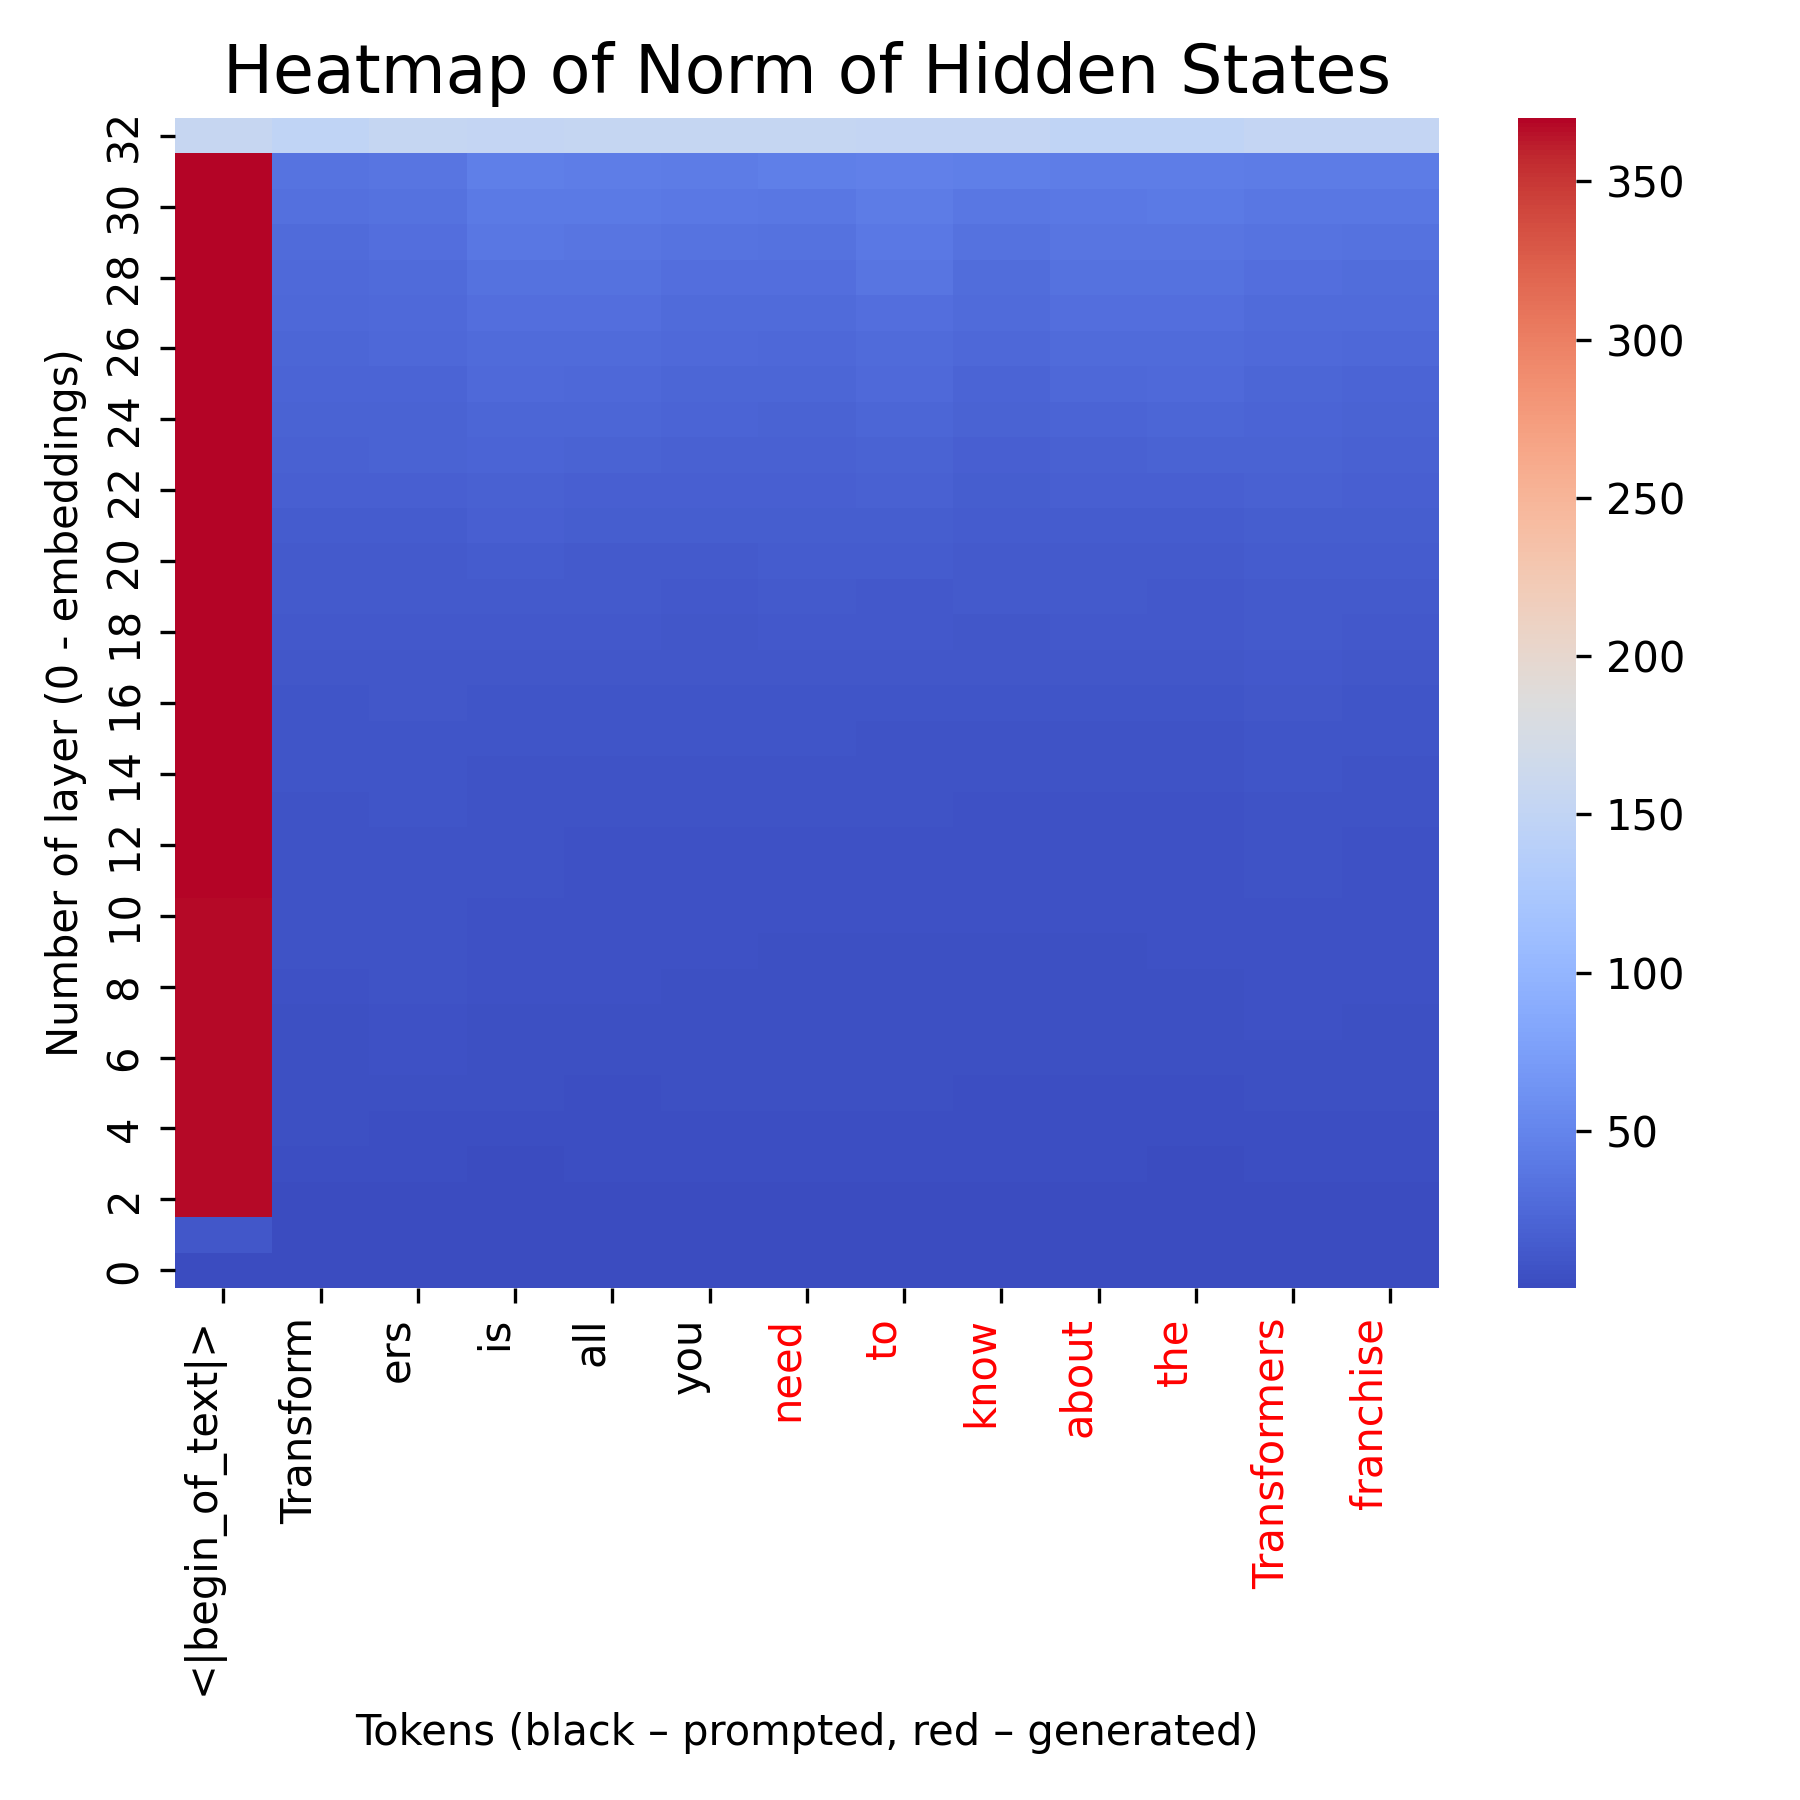
\includegraphics[width=\textwidth]{images/heatmap_8b_full.png}
        \caption{Heatmap of hidden state norms across layers and tokens for Llama 3.1 8B model. The x-axis represents tokens in the sequence (with generated tokens in red), and the y-axis represents model layers (with 0 being the embedding layer). Brighter colors indicate larger norms.}
        \label{fig:heatmap_8b_full}
    \end{minipage}
    \hfill
    \begin{minipage}{0.48\textwidth}
        \centering
        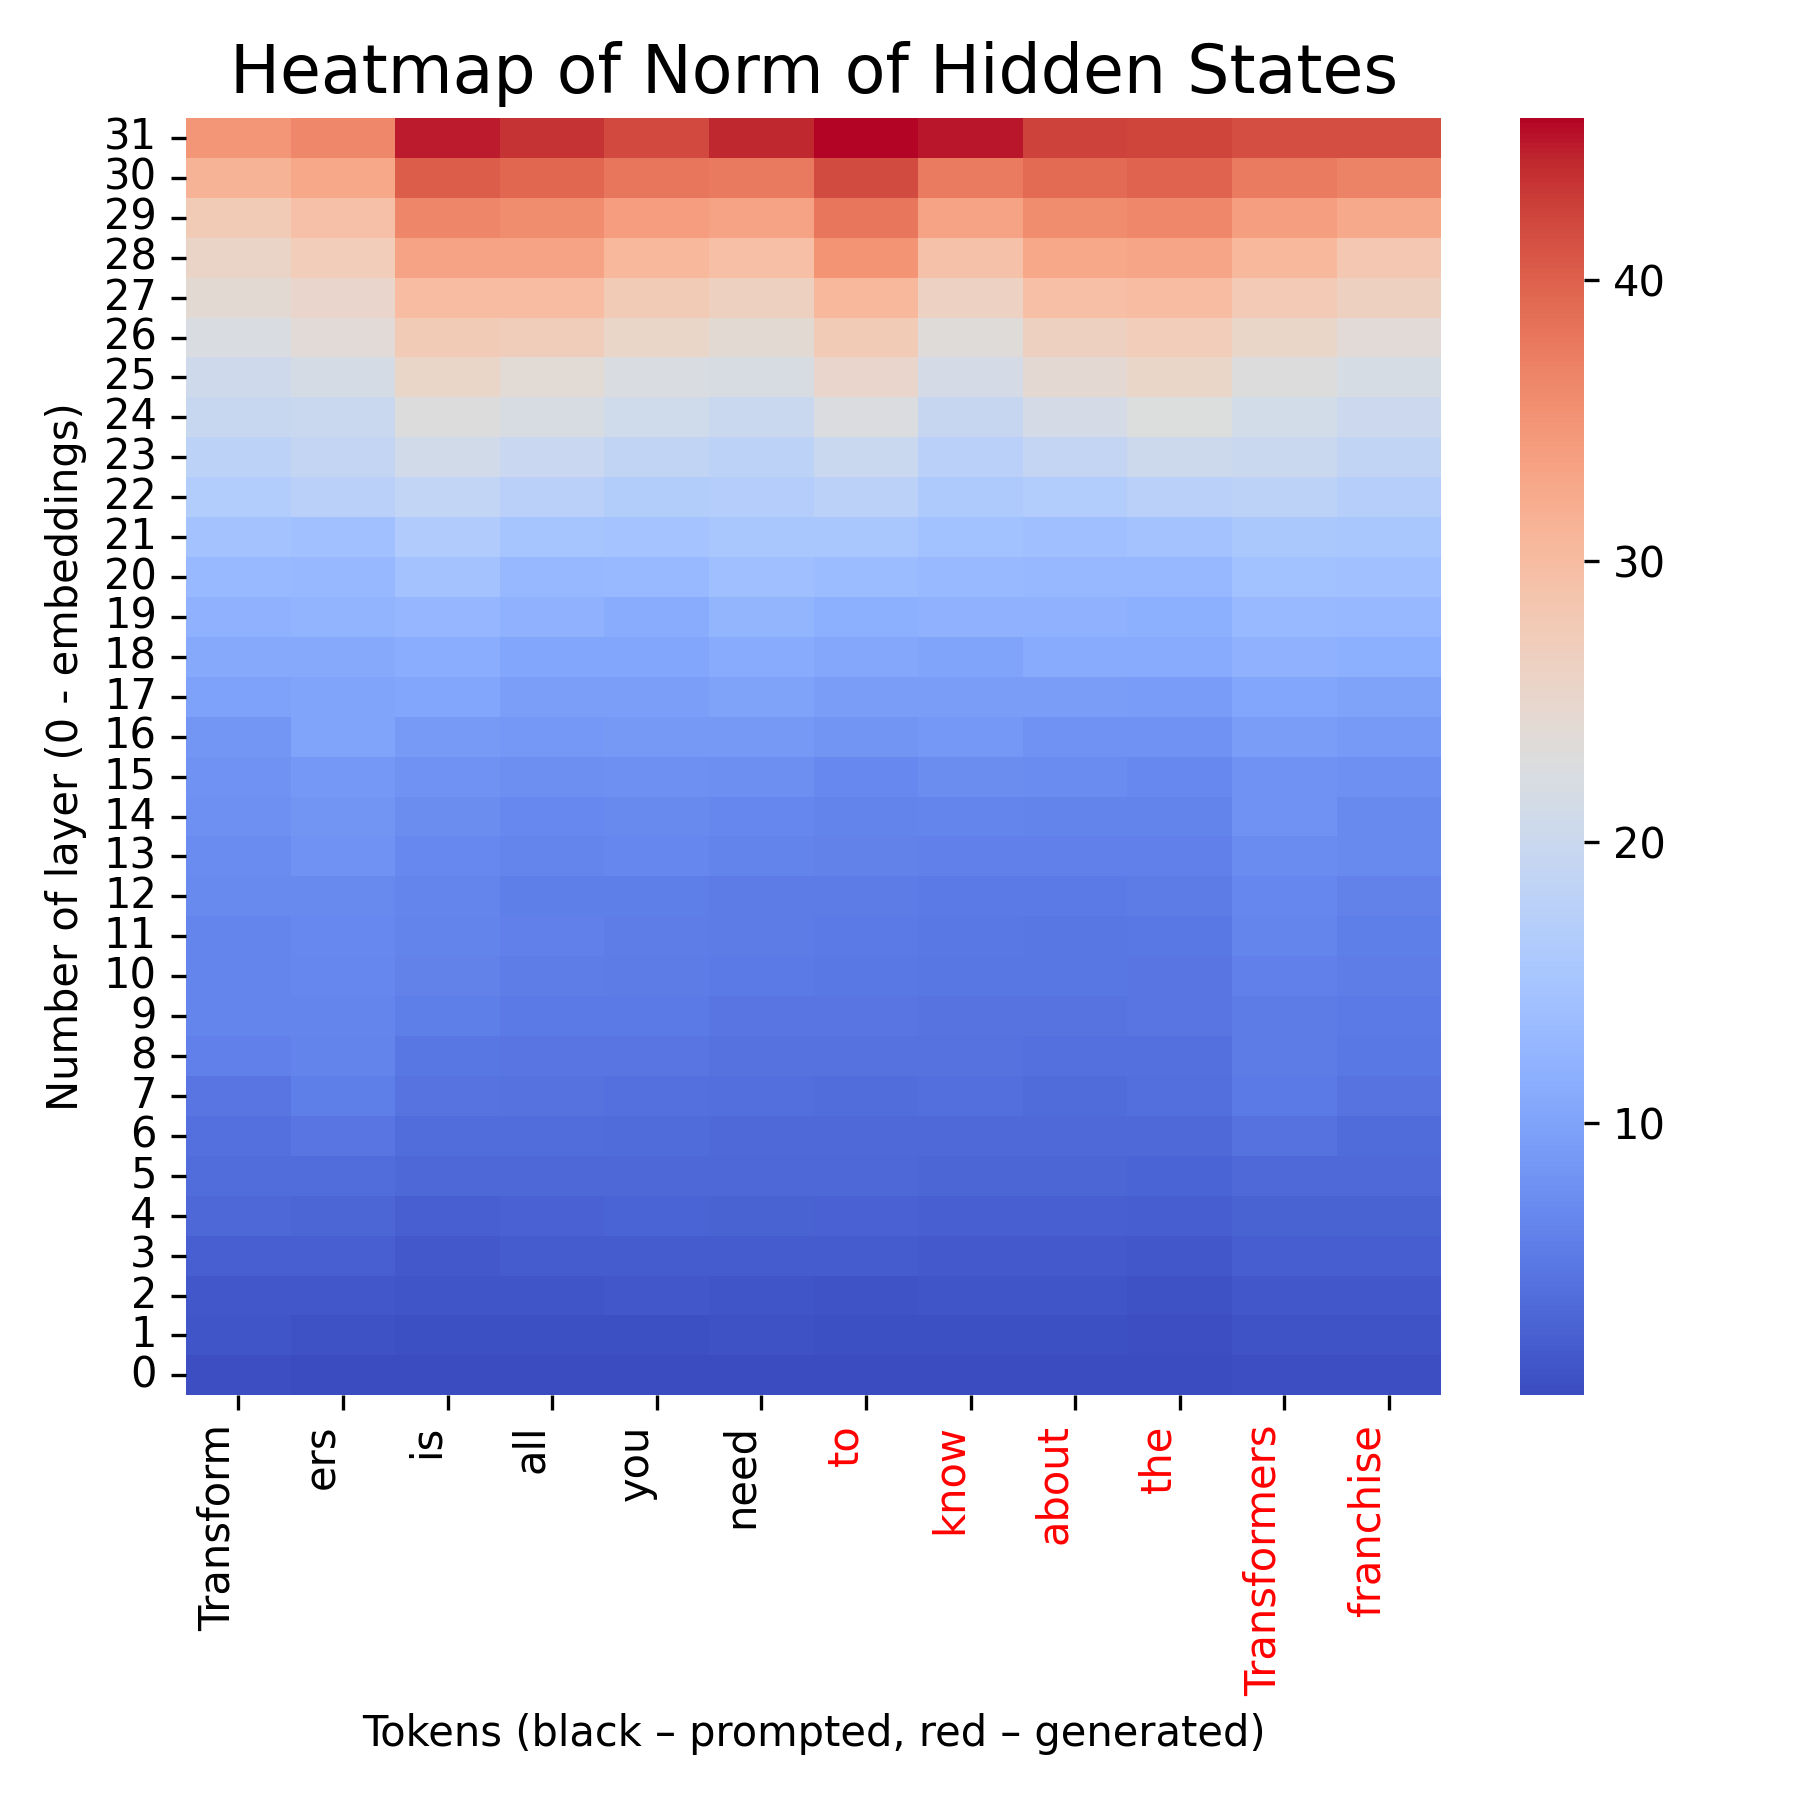
\includegraphics[width=\textwidth]{images/heatmap_8b_notfull.png}
        \caption{Heatmap of hidden state norms excluding the <BOS> token and final layer for Llama 3.1 8B model, providing a clearer view of the norm distribution in intermediate layers. Note the gradual increase in norm magnitude as layer depth increases.}
        \label{fig:heatmap_8b_notfull}
    \end{minipage}
\end{figure}

\begin{figure}[h]
    \centering
    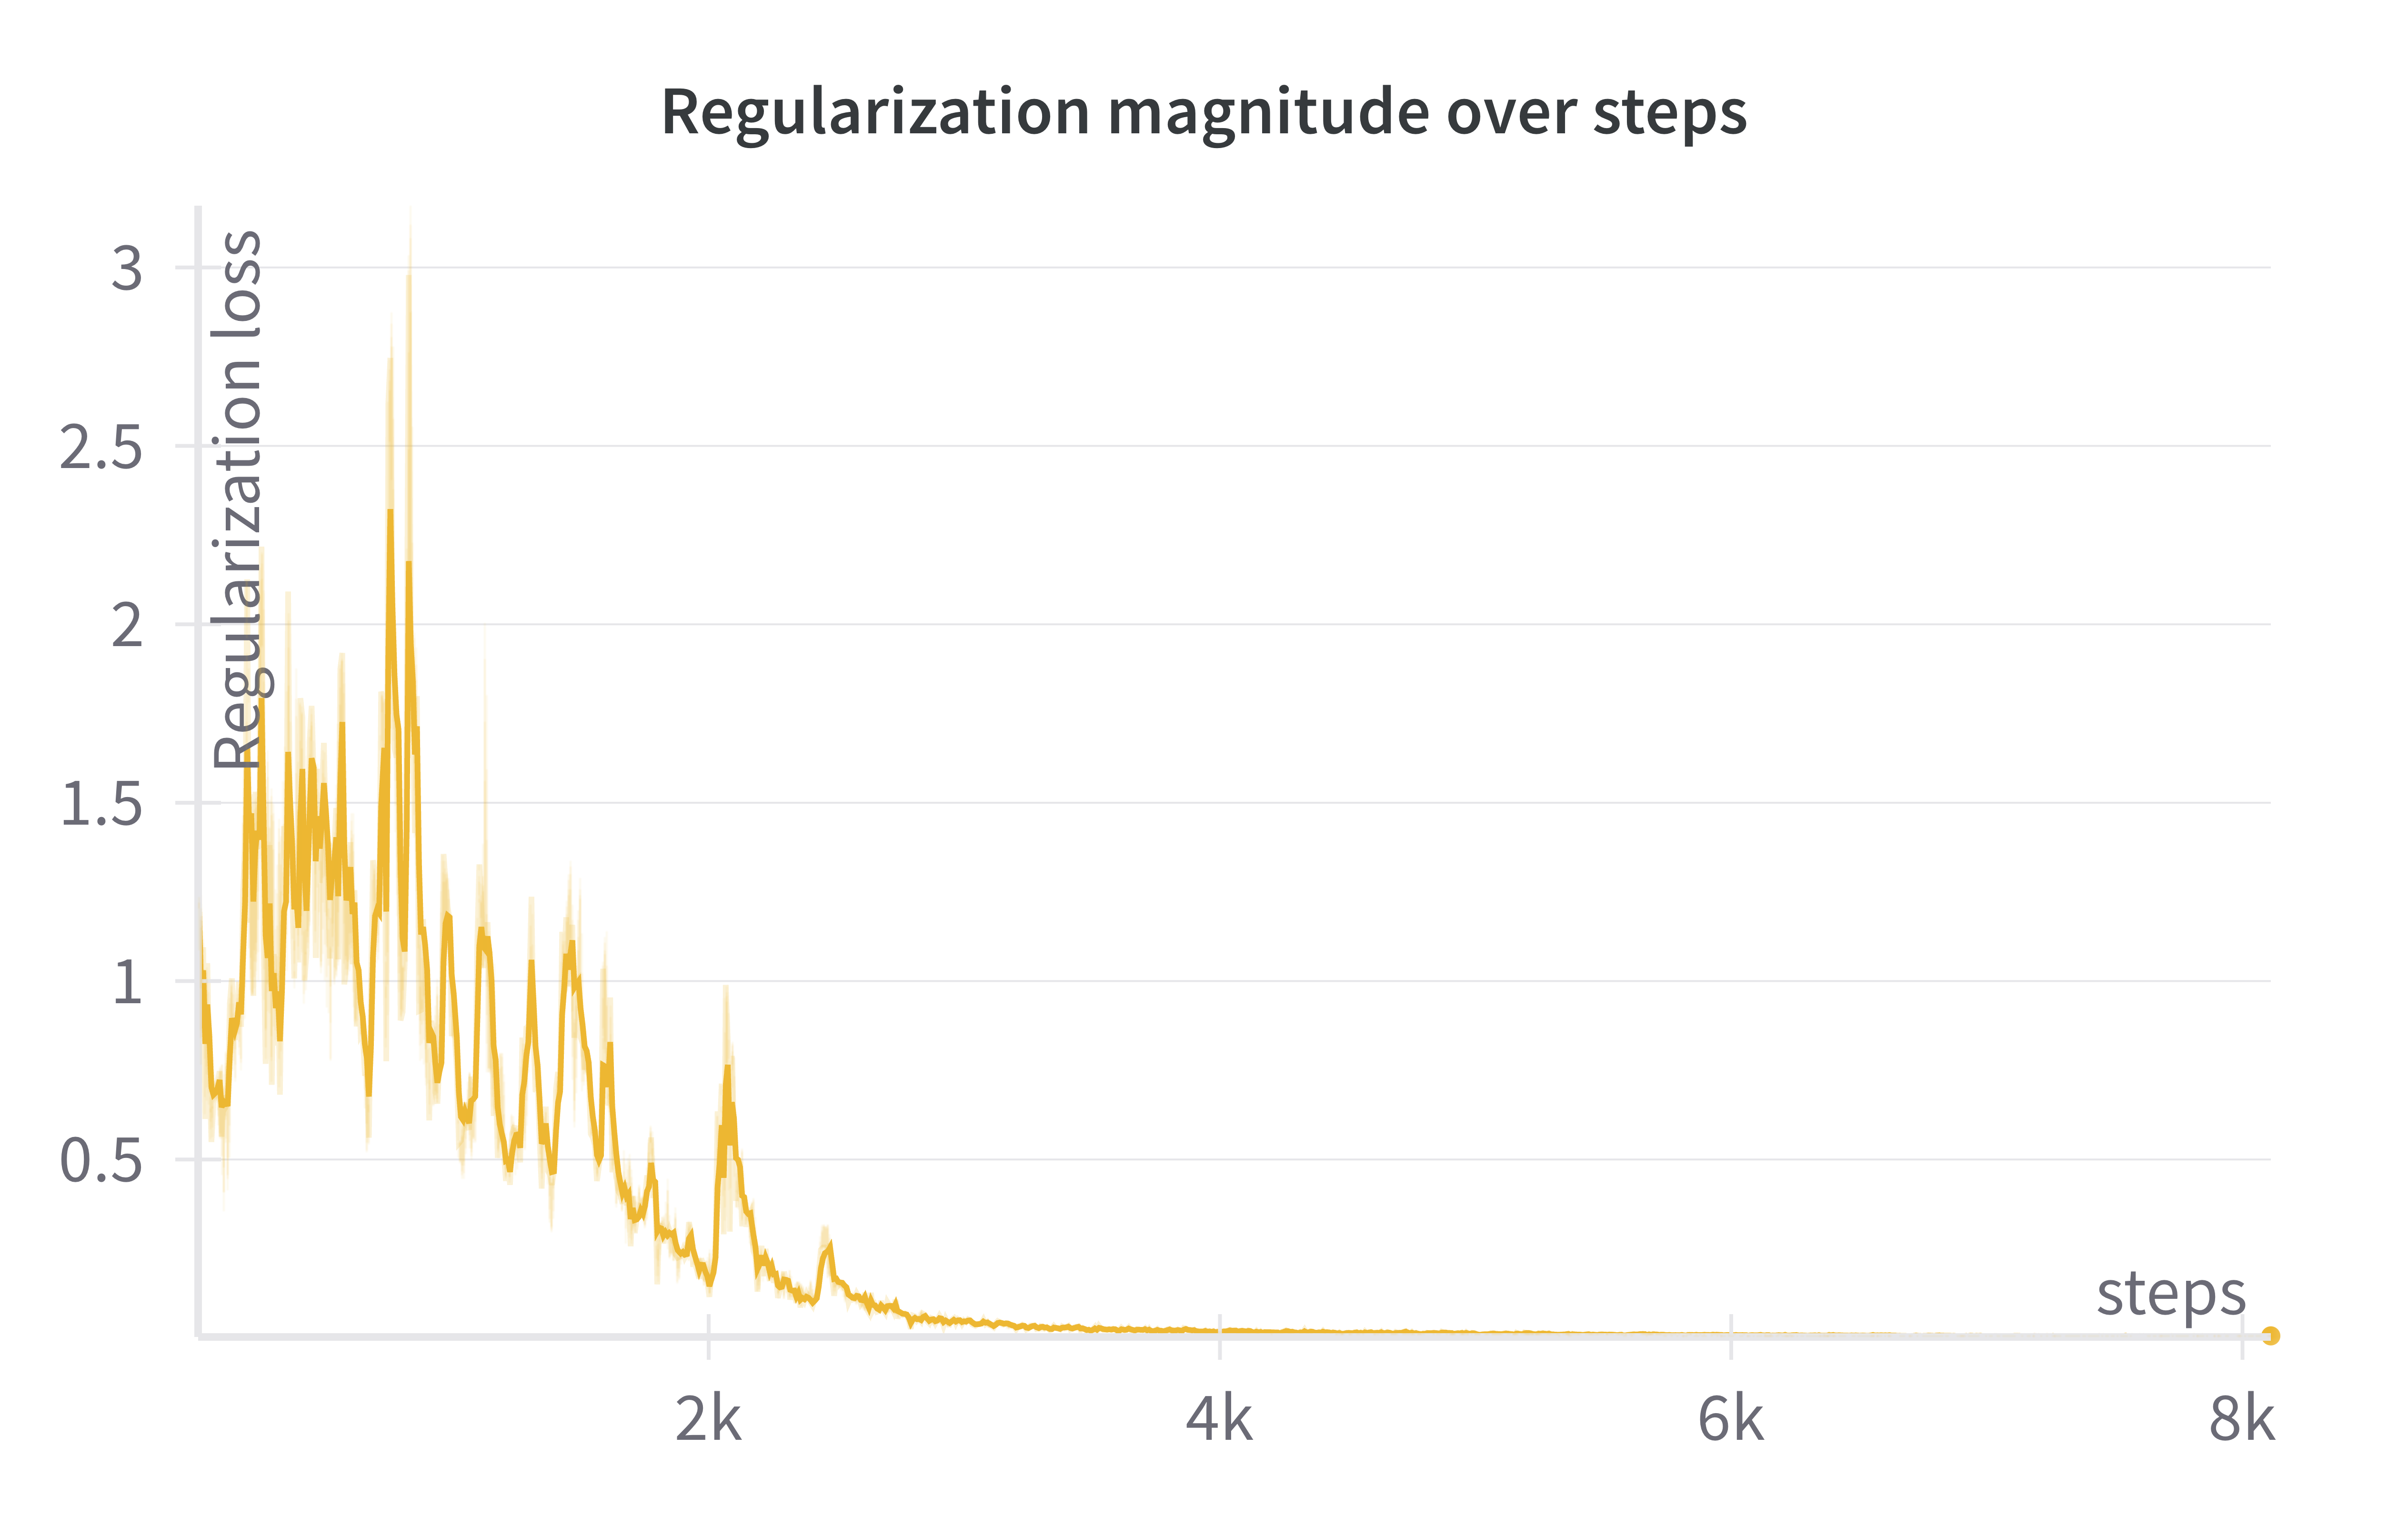
\includegraphics[width=0.7\textwidth]{images/reg_loss.png}
    \caption{Regularization magnitude over steps during training. At the beginning of training, the regularizing penalty kick contributes significantly to the loss. However, as training progresses, its impact decreases and it becomes negligible.}
    \label{fig:reg_loss}
\end{figure}

